
\section[Листинг программы расчёта ФСС]{обязательное}\label{app:matlab_fss}
%\sectionmark{Пример работы совместно с Matlab}

%\lstinputlisting[style=MatlabStyle, showspaces=false]{./content/FiltrPH.m}

%\begin{minted}[breaklines]{c}
%int main() {
%printf("hello, world");
%return 0;
%}
%\end{minted}



\begin{figure}[H] \centering
  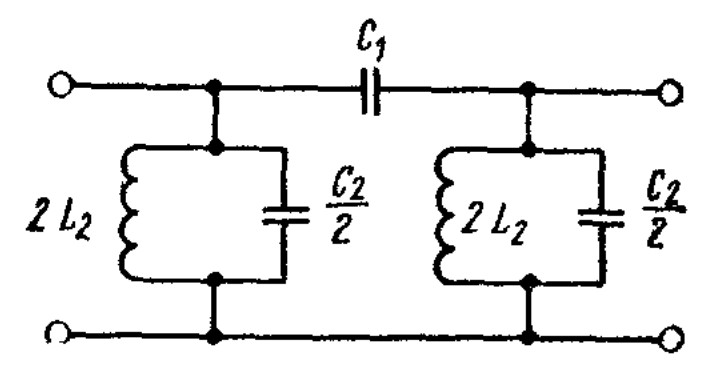
\includegraphics[width=0.8\textwidth]{./content/Sivers_filter.jpg}
  \caption{Звено фильтра сосредоточенной селекции \cite{Sivers}, c. 283. } \label{p:Sivers_filter}
\end{figure}





%\begin{minted}{c}
\inputminted[fontsize=\small, linenos, breaklines, numbersep=2mm, xleftmargin=5mm]{matlab}{./content/FiltrPH.m}
%\end{minted}



\section[Листинг программы расчёта входной цепи с индукнтивно-емкостной связью]{обязательное}\label{app:matlab_vplc}


\begin{figure}[H] \centering
  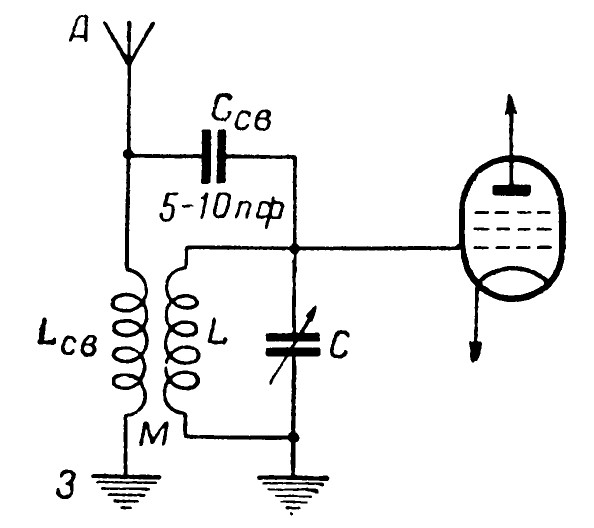
\includegraphics[width=0.8\textwidth]{./content/Siforov_20.jpg}
  \caption{Схема с индуктивно-емкостной связью между контуром и антенной  \cite{Siforov}, c. 35. } \label{p:Siforov_20}
\end{figure}



\inputminted[fontsize=\small, linenos, breaklines, numbersep=2mm, xleftmargin=5mm]{matlab}{./content/VhCerkets3_1.m}

